\section{Infrastruktur}
\label{Infrastruktur}

\subsection{Entwicklungsumgebung}
Als \ac{IDE} wurde für dieses Projekt Android Studio 1.4 eingesetzt. Android Studio basiert auf IntelliJ und hat Ende 2014 die \enquote{Eclipse Android Development Tools} als Standard \ac{IDE} für Android Projekte abgelöst.\cite{android_studio_stable}

Für die Versionsverwaltung wurde Git mit einem Projekt Repository der \ac{HSR} (\url{git.hsr.ch}) verwendet. Lokal wurde der grafische Git-Client SourceTree benutzt.

Um Continuous Integration zu ermöglichen haben wir zusätzlich auf einem \ac{VPS} der \ac{HSR} einen Jenkins Build-Server eingerichtet. Der Build-Server prüft mittels Polling ob neue Commits vorhanden sind und kompiliert gegebenenfalls jeweils eine neue Version der Applikation. So wird sichergestellt, dass eine Änderung nicht nur lokal kompiliert, sondern überall. Zudem bietet der Build-Server die Möglichkeit, die jeweils aktuellste Version der Applikation an Tester zu verteilen.

\subsection{Projektmanagement}

Zur Unterstützung des Projektmanagements wurde Redmine auf dem \ac{VPS} der \ac{HSR} eingerichtet. Vor allem die von Redmine gebotenen Funktionen Issue Verwaltung, Gantt Diagramm, Wiki und File-Repository wurden intensiv eingesetzt.

\subsection{Testgeräte}

Von der \ac{HSR} wurden uns zwei Android Smartphones zur Verfügung gestellt. Ein \enquote{LG Nexus 5} mit Android 6.0 sowie ein \enquote{Samsung Galaxy Nexus} mit Android 4.3. Mit dem \enquote{Samsung Galaxy Nexus} decken wir die Mindestanforderungen der Applikation (API Level 18 - Android 4.3) ab und mit dem \enquote{LG Nexus 5} wird sichergestellt dass die Applikation auch auf Geräten mit der neusten Android Version (Stand Dezember 2015) läuft.

Zum simulieren der Küchengeräte erhielten wir von Fluxron einen Testaufbau. Dieser besteht aus drei Bluetooth Controllern wie sie bei Induktionsheizgeräten eingesetzt werden.

\begin{wrapfigure}[15]{l}{9cm}
	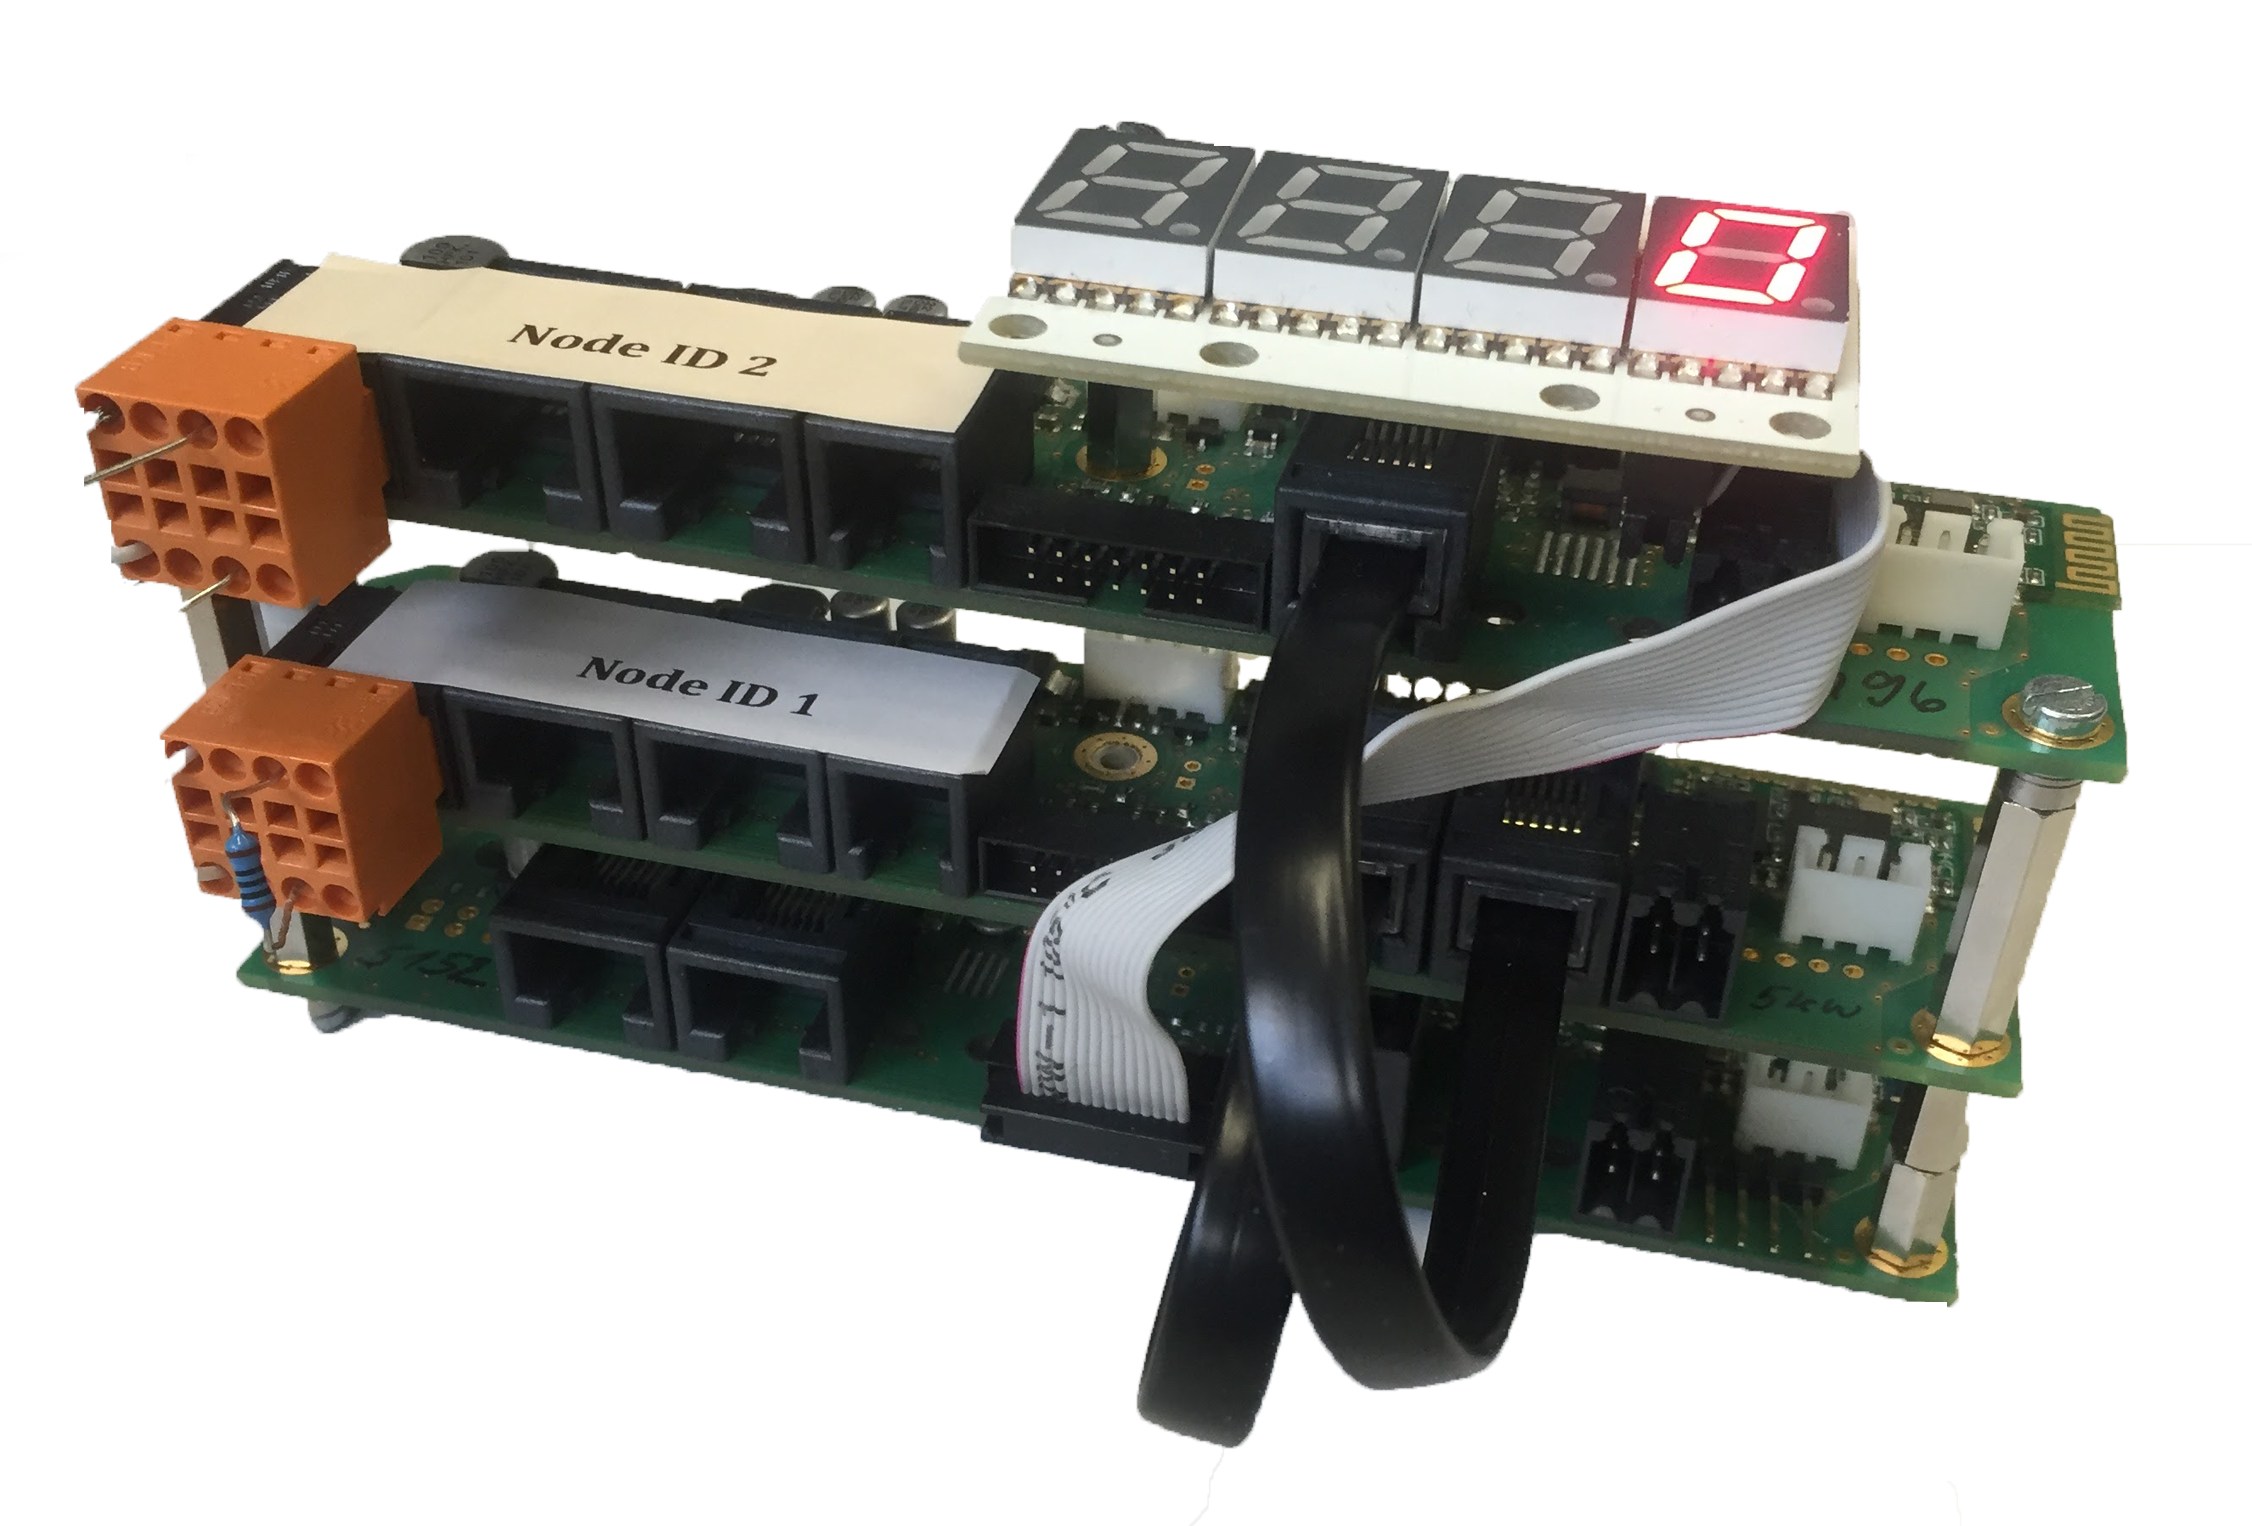
\includegraphics[scale=0.1025]{appendix/res/fluxron_device_transparent}
	\caption{Fluxron Testaufbau}
\end{wrapfigure}

\ 

\begin{enumerate}
\item \textbf{Revision:} C-Class\\ \textbf{Typ:} BAX\\ \textbf{Bluetooth:} Classic\\
\item \textbf{Revision:} C-Class\\ \textbf{Typ:} REX\\ \textbf{Bluetooth:} Classic\\
\item \textbf{Revision:} C-Class\\ \textbf{Typ:} BAX\\ \textbf{Bluetooth:} Classic \& 4.0
\end{enumerate}
